\documentclass[journal]{IEEEtran}

%\usepackage{cite}

\usepackage{graphicx}

\usepackage{wrapfig}

\usepackage{hyperref}  

\hypersetup{
	colorlinks,
	citecolor=black,
	filecolor=black,
	linkcolor=cyan,
	urlcolor=blue
}

%\usepackage{amsmath}

\interdisplaylinepenalty=2500

%\usepackage{array}

%\usepackage[english]{babel}

\usepackage{caption}

\usepackage{subcaption}

\usepackage{float}

%\usepackage{biblatex}

%\addbibresource{myref.bib}

\setlength{\parskip}{0.5em}  

\begin{document}
	\title{Week 1 Journal and In-Class Assignments}
	
	\author{{\LARGE Submitted by: Dhiraj~Gharana}\\{\large Submitted to: Dr. Boult (CS 6000)}\\ {\normalsize ~University~of~Colorado~at~Colorado~Springs}}
	
	\markboth{Week 1 Journal: \today}
	{This heading will be blocked by the page numbers...}
	
	\maketitle
	
\section{Biography}
\label{sec:biography}
	
\noindent I'm from Nepal, a country in Asia flanked on either side by India and China. Currently, I am remotely pursuing a Ph.D. in Engineering (concentration in Computer Science) at the University of Colorado at Colorado Springs (UCCS).    	   
	
\begin{wrapfigure}{r}{0.4\linewidth}
	\begin{center}
		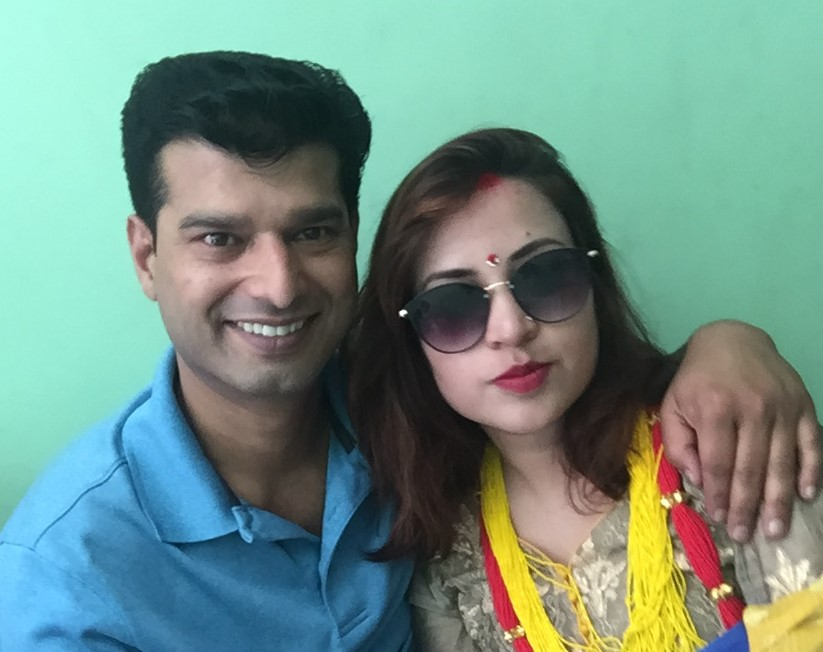
\includegraphics[width=0.9\linewidth]{images/fig1}
	\end{center}		
	\caption*{\footnotesize My wife, a medical doctor, and I a few months after our marriage. The necklaces she is wearing are the traditional necklaces worn by wives in Nepal. She is also wearing a vermilion red cosmetic powder called ``Sindoor,'' which Hindus believe will bestow longevity and health on her husband. Though I only believe in mathematics and science, I appreciate her display of affection and love.}		
\end{wrapfigure}  

\noindent Recently, I have been working on a survey paper by the name ``A synopsis of cross-situational word learning (CSWL) in robots: with insights from CSWL research in young children,'' under the supervision of Dr. Jugal Kalita \footnote{Dr. Jugal Kalita is the Chair of the Computer Science Department of the College of Engineering and Applied Sciences at UCCS.}. My computer science research goal is to find better solutions to the problem of robots learning natural languages through multi-modal perception across different contextual situations while conversing and interacting with humans.  

\noindent Apart from research in computer science, I am also interested in contributing to the human endeavor of understanding the mechanisms of strong natural emergence, in which the interaction of a massive collection of microscopic (smaller) entities gives rise to a macroscopic system with new properties and functionalities that were not present in any given single microscopic constituent. Examples of strong natural emergence include the formation of atoms and chemical bonds from the interaction of sub-atomic particles, the creation of multi-cellular organisms, like humans, from the interaction of a myriad of cells, and the existence of an ecosystem from the interaction of many living organisms residing in the biosphere of earth, and more interestingly, the emergence of consciousness due to the interaction of many neurons in the human brain.  

\subsection{Goals for This Course}   
\label{sec:coursegoals}  

\noindent As will be evident from the description provided in section \ref{sec:lessonslearned}, my initial approach to research cost me significantly in time and effort.  

\noindent After taking this course by Dr. Boult \footnote{Dr. Boult is El Pomar Endowed Professor of Innovation and Security at UCCS, co-director of the Bachelor of Innovation family of degrees, the chair of the IEEE PAMI Technical Committee, and a founding member of the IEEE Biometrics Council.} I hope to learn the canons and the caveats with respect to Computer Science Research so as to develop a cost-effective approach to surveying the literature relevant to my research at hand, to adopt an apt general protocol for conducting, collaborating on, and evaluating research, and to acquaint myself with proper research writing skills and also with the different journals and venues in which I can attempt to publish my work. I am sure that this course will also introduce tools that will prove useful, if not indispensable, to optimally conducting and sharing my research work.   

\noindent In addition to gaining pertinent knowledge and learning useful skills related to the solution space, as mentioned in the previous paragraph, I believe this course will also guide me in regard to identifying and choosing a proper research problem to pursue and will facilitate my understanding of the various constraints, limitations, and intricacies of the problem space.        

\subsection{Research Publications}
\label{sec:publications}  

D. Gharana, S. C. Suh, and M. Kang, ``Gender classification based on deep learning'' in \textit{Big Data and Visual Analytics}, 1st Ed. S. C. Suh, T. Anthony, Eds. Springer International Publishing, 2017, ch. 3, pp. 55–69, doi: 10.1007/978-3-319-63917-8.  

D. Gharana, ``Gender and age classification from facial images using deep learning'' M.S. thesis, College of Sc. and Eng., Texas A \& M University - Commerce, Texas, U.S.A, July. 2016.  

\subsection{Academic and Research Lessons Learned}   
\label{sec:lessonslearned}

\begin{quote}
	``\textit{Reading without thinking is useless. Thinking without reading is dangerous.}''
	
	\raggedleft
	--\ \footnotesize Confucius, taken from goodreads, where I replaced `learning' by `reading' \\ \tiny \textbf{\textit{https://www.goodreads.com/quotes/9059465-learning-without-thinking-is-useless-thinking-without-learning-is-dangerous}}
\end{quote}

\noindent Any PhD researcher needs to read extensively. Yet, simply reading a lot does not guarantee
erudition. Mental retention of facts and acquisition of knowledge are meaningful only if that
knowledge can be applied to solve real-life problems. On the other hand, in addition to innovative thinking, successful research depends heavily on acquaintance to others' work through extensive literature review and collaboration.  

\noindent The initial part of the above quote is relevant to my undergraduate academic pursuits as I learned from my freshman year that reading for exams and other coursework without an in-depth understanding of the concepts being studied and a vision of how these concepts relate to other previously mastered concepts, never helped me master the subject matter so as to be able to solve real life problems. Consequently, I abandoned this approach early on during my undergraduate studies.  

\noindent The latter part of the above quote is relevant to my early graduate research endeavors in that zealously pursuing innovative ideas with a dearth of literature review often lead to the duplication of already published work, the cumbersome chore of re-inventing the wheel, the malpractice of coining new terms for technical concepts that already exist in the jargon of published work, and the almost inevitable consequence of having to eventually abandon my research endeavor.  

\noindent However, I now acknowledge literature review as the most important initial step in understanding the problem at hand and exploring known solutions; the fact that my book chapter research publication is replete with references corroborates this claim.  

\section{Learning from this week: {\normalsize $09/02 \; - \; 09/08$ }}
\label{sec:learning}  

\subsection{My Git Repository}  
\label{sec:gitrepo}  
  
\noindent I have a public git repository on GitHub for this course. The following is the url of the repository: {\footnotesize  \textbf{https://github.com/scientiagharana/Dhiraj-Gharana-Dr-Boult-CS6000.git}} \href{https://github.com/scientiagharana/Dhiraj-Gharana-Dr-Boult-CS6000.git}{Dhiraj-Gharana-Dr-Boult-CS6000}  

\subsubsection{The Tools Used}  
\label{sec:toolsused}

\noindent I installed git on my system (Windows 10) and then I created the git repository, mentioned in section \ref{sec:gitrepo}, online using GitHub.  I then cloned the git repository onto my personal system and created the folder ``Assignments and Journals,'' into which I have placed this document. I committed my local changes and then pushed them to the master branch.      

\subsection{My Learning}
Below, I list the main concepts and skills I learned from this course this week:  

\begin{enumerate}
	\item I learned the qualities a scholarly endeavor must possess in order to qualify as good research.  
	\item I learned the different approaches used for research in Computer Science.  
	\item I learned how to use Google Scholar effectively as a research journal search and scan tool.  
	\item I learned how to evaluate research papers and how to use Google Scholar to view the citation count for any research paper.  
	\item I was already familiar with Mendeley. Nonetheless, this week I learned about Zotero as a potential alternative for reference management.  
	\item I learned a bit more about LaTeX and about using LaTeX to write theses and dissertations. However, I have already written research articles in LaTeX using different journal templates and am already adept at using it for simple research writing.  
	\item This course also taught me the benefits of using Overleaf, especially the Overleaf online LaTeX editor. However, I still prefer writing LaTeX documents offline using TeXstudio's editor, with MiKTeX (the LaTeX typesetting system for Windows), on my own system.  	   
\end{enumerate}  

\subsection{Problems and Struggles}  

\subsubsection{A research idea becomes research only when shared}  

In the first video for Lecture 1, Dr. Boult states --- research work that is not shared can qualify as merely a research idea and not as research.    

\section{Papers Relevant to My Research}  



\section{In-Class Exercises Related to Lecture 1}
\label{sec:inclassexercises}   

\subsection{Google Scholar Exercises}  
\label{sec:googlescholar}

\subsubsection{Finding A Relevant Research Paper}

The research topic I am interested in is ``Cross-situational word learning (CSWL) in robots: inspired by CSWL research in young children.''

I ran the search key phrase ``cross-situational word learning in robots,'' without quotes, on Google Scholar and obtained the following result.  

\begin{figure}[H]
	\begin{center}
		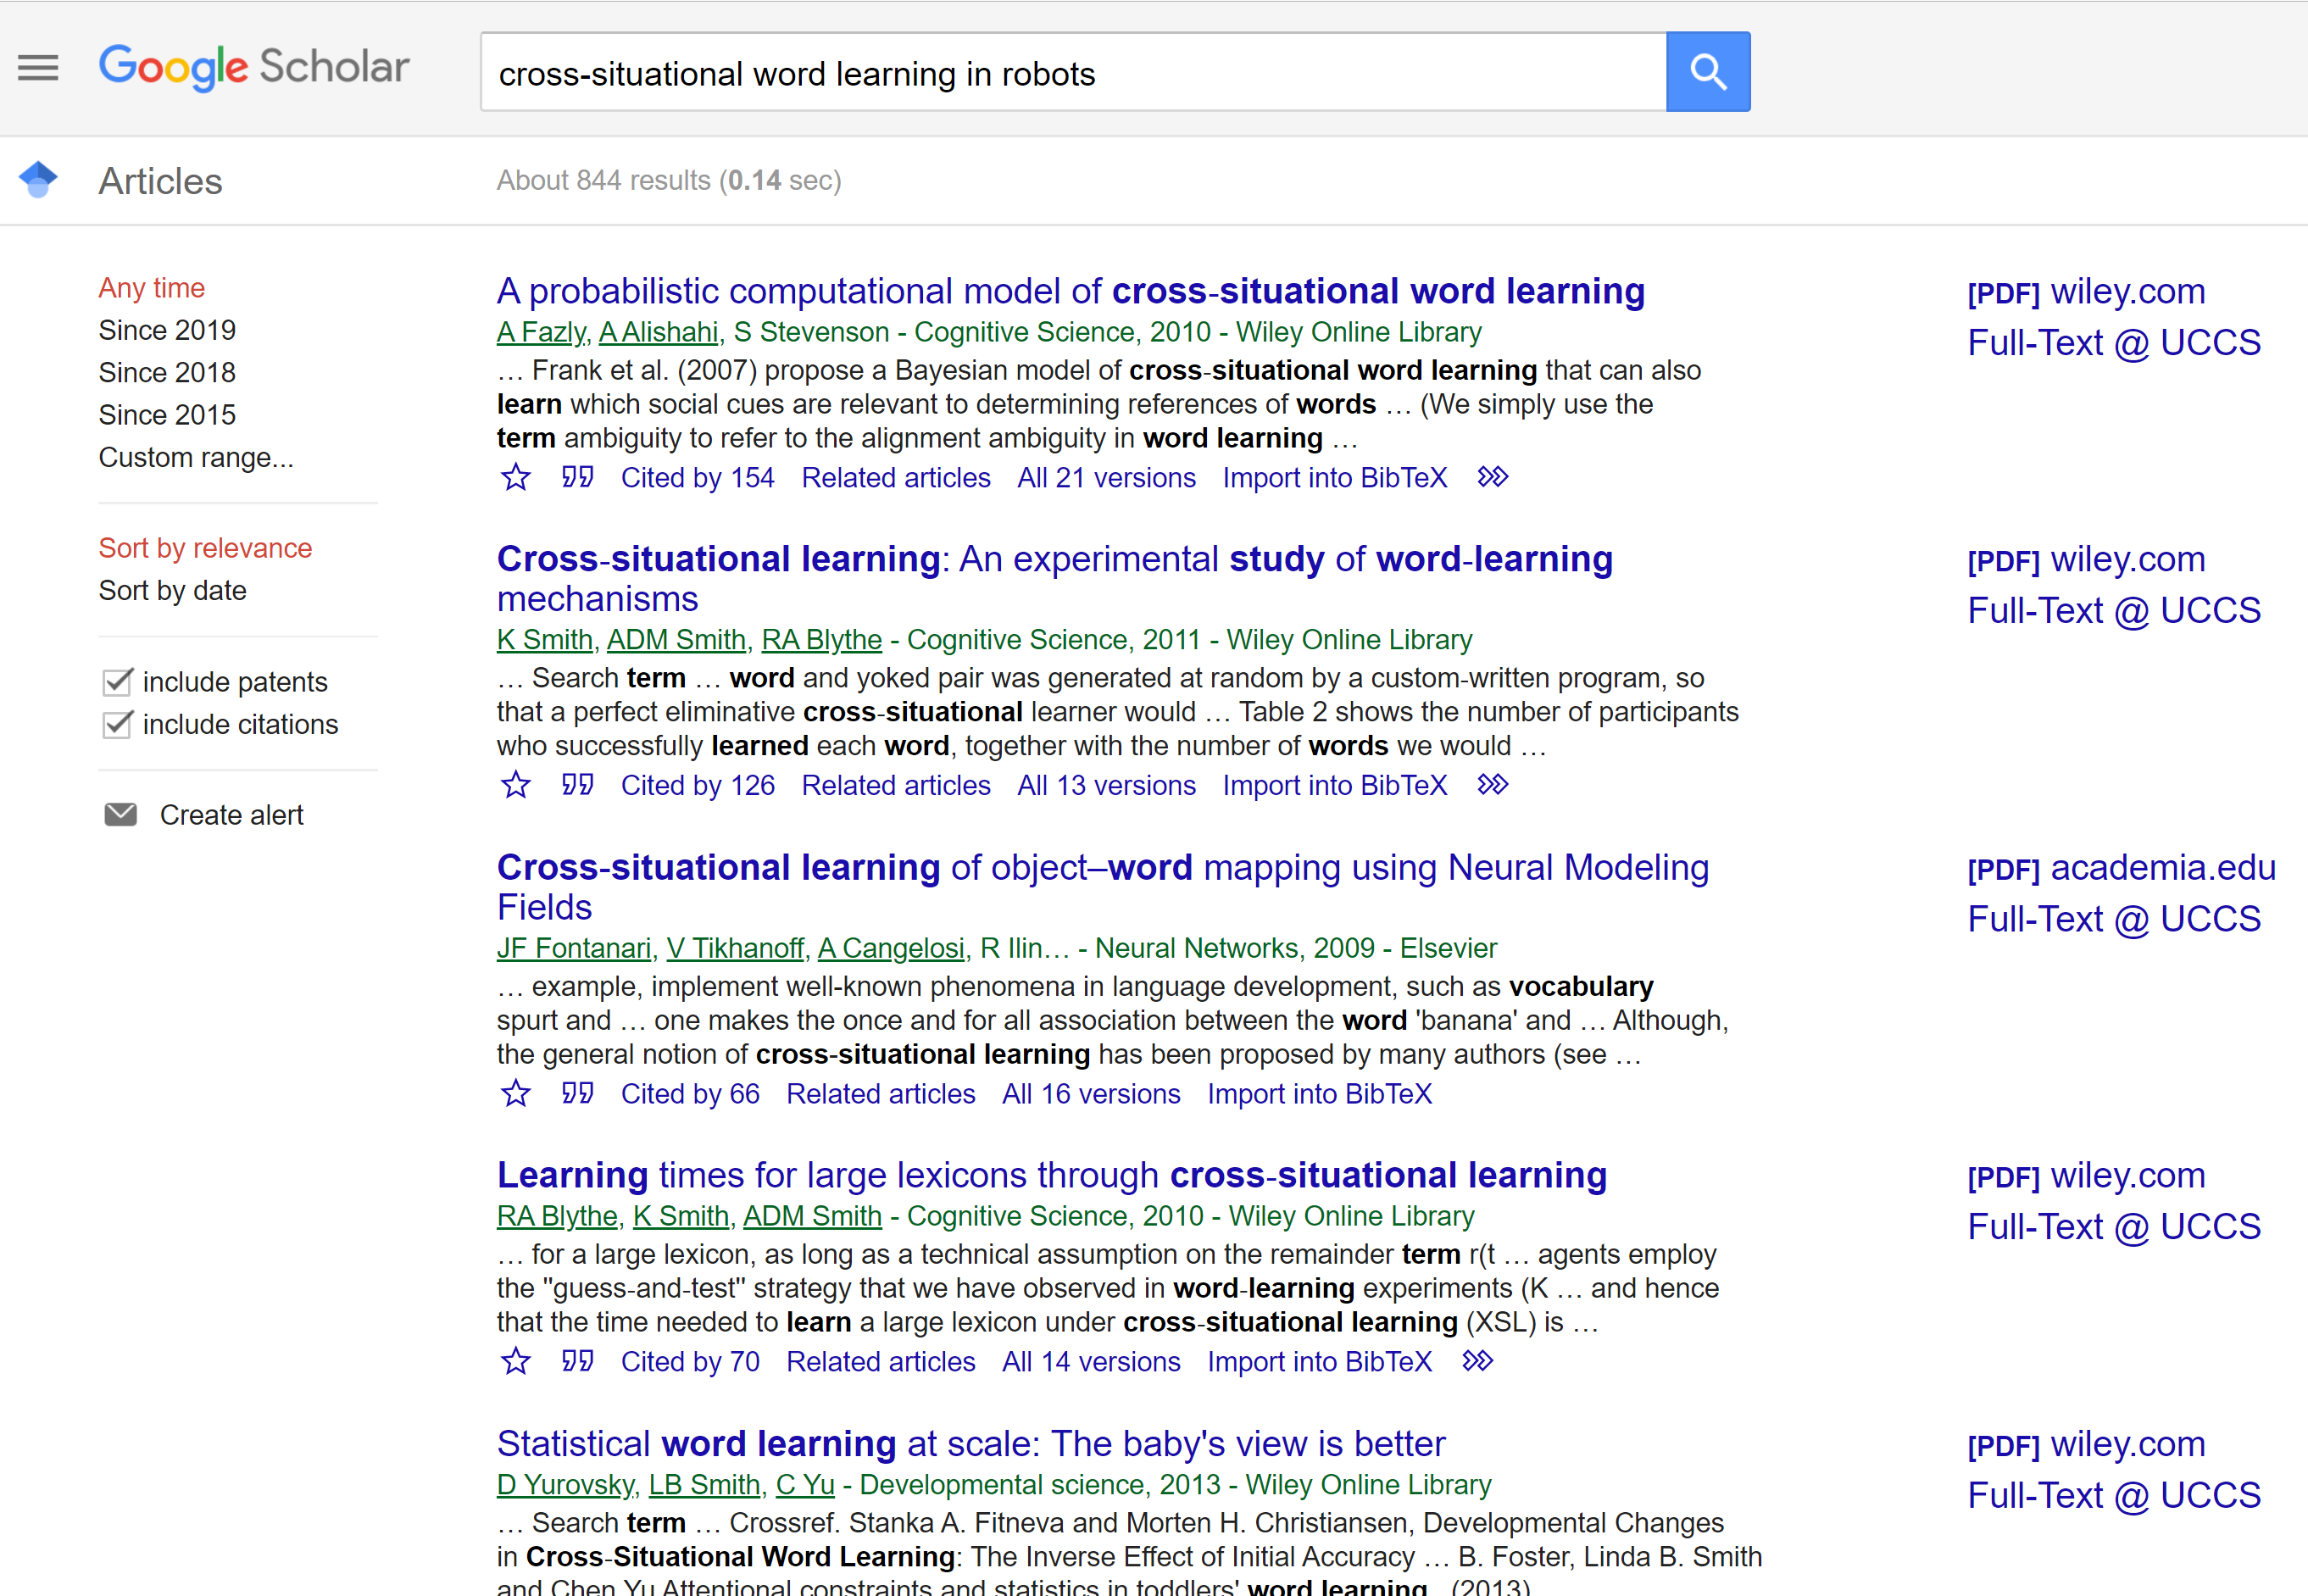
\includegraphics[width=0.9\linewidth]{images/fig3}
	\end{center}
	\captionsetup{labelformat=empty}
\end{figure}  

Interestingly, four out of the first five results rendered by Google Scholar, all shown in the figure above excluding ``Learning times for large lexicons through cross‐situational learning,'' were very relevant to the survey paper I am writing.  

I have used IEEE Xplore, ScienceDirect, and Semantic Scholar to search for journal articles in the past. I am grateful that this course demonstrated the benefits of using Google Scholar for this purpose. I feel I will be using Google Scholar quite frequently from now on.      

\subsubsection{Finding Most Cited Papers by My Supervisor}  

My research supervisor is Dr. Jugal Kalita.  

I typed author:"J. Kalita" into the basic search of google scholar, which presented me with two authors to select from, shown below.  

\begin{figure}[H]
	\begin{center}
		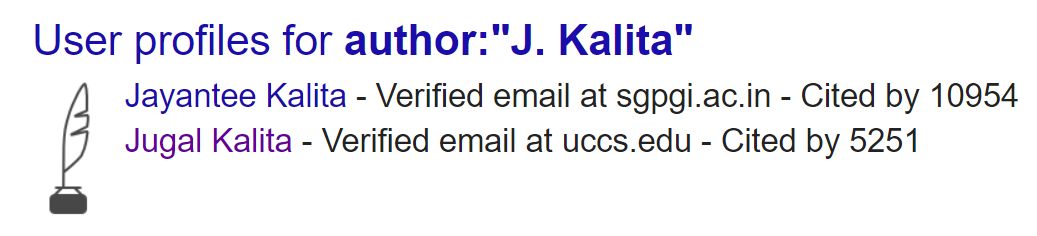
\includegraphics[width=0.9\linewidth]{images/fig2}
	\end{center}
	\captionsetup{labelformat=empty}
\end{figure}  

I clicked on my supervisor's name, Jugal Kalita, and reached his profile page, which has his papers sorted by number of citations \footnote{I assume that the greater the number of citations a paper receives, the better the quality of research presented in that paper}.  
The following shows a list of the first few papers listed in Dr. Jugal Kalita's profile page according to their citation ratings.      

\begin{center}
	\begin{tabular}{ |l|c|r| } 
		\hline
		{\footnotesize \textbf{Title}} & {\footnotesize \textbf{Cited by}} & {\footnotesize \textbf{Year}}\\
		\hline
		{\tiny Network anomaly detection: methods, systems and tools \cite{article157}} & {\tiny 622} & {\tiny 2013} \\ 
		\hline
		{\tiny Summarizing microblogs automatically \cite{article158}} & {\tiny 240} & {\tiny 2010} \\ 
		\hline
		{\tiny Syntactic normalization of twitter messages \cite{article159}} & {\tiny 195} & {\tiny 2010} \\ 
		\hline		
	\end{tabular}
\end{center}  

\subsubsection{Finding Select Papers Written by Dr. Boult}  

To find articles authored by \textbf{Dr. Terrance Boult}, the instructor of this course, published in \textit{IEEE Transactions on Pattern Analysis and Machine Intelligence} within the past five years, I used the Advanced Search option of Google Scholar as shown below:  

\begin{figure}[H]
	\begin{center}
		
\includegraphics[width=0.9\linewidth]{images/fig4}
	\end{center}
	\captionsetup{labelformat=empty}
\end{figure}   

The three results, which seems to be the exhaustive list, rendered by Google Scholar is provided below:  

\begin{figure}[H]
	\begin{center}
		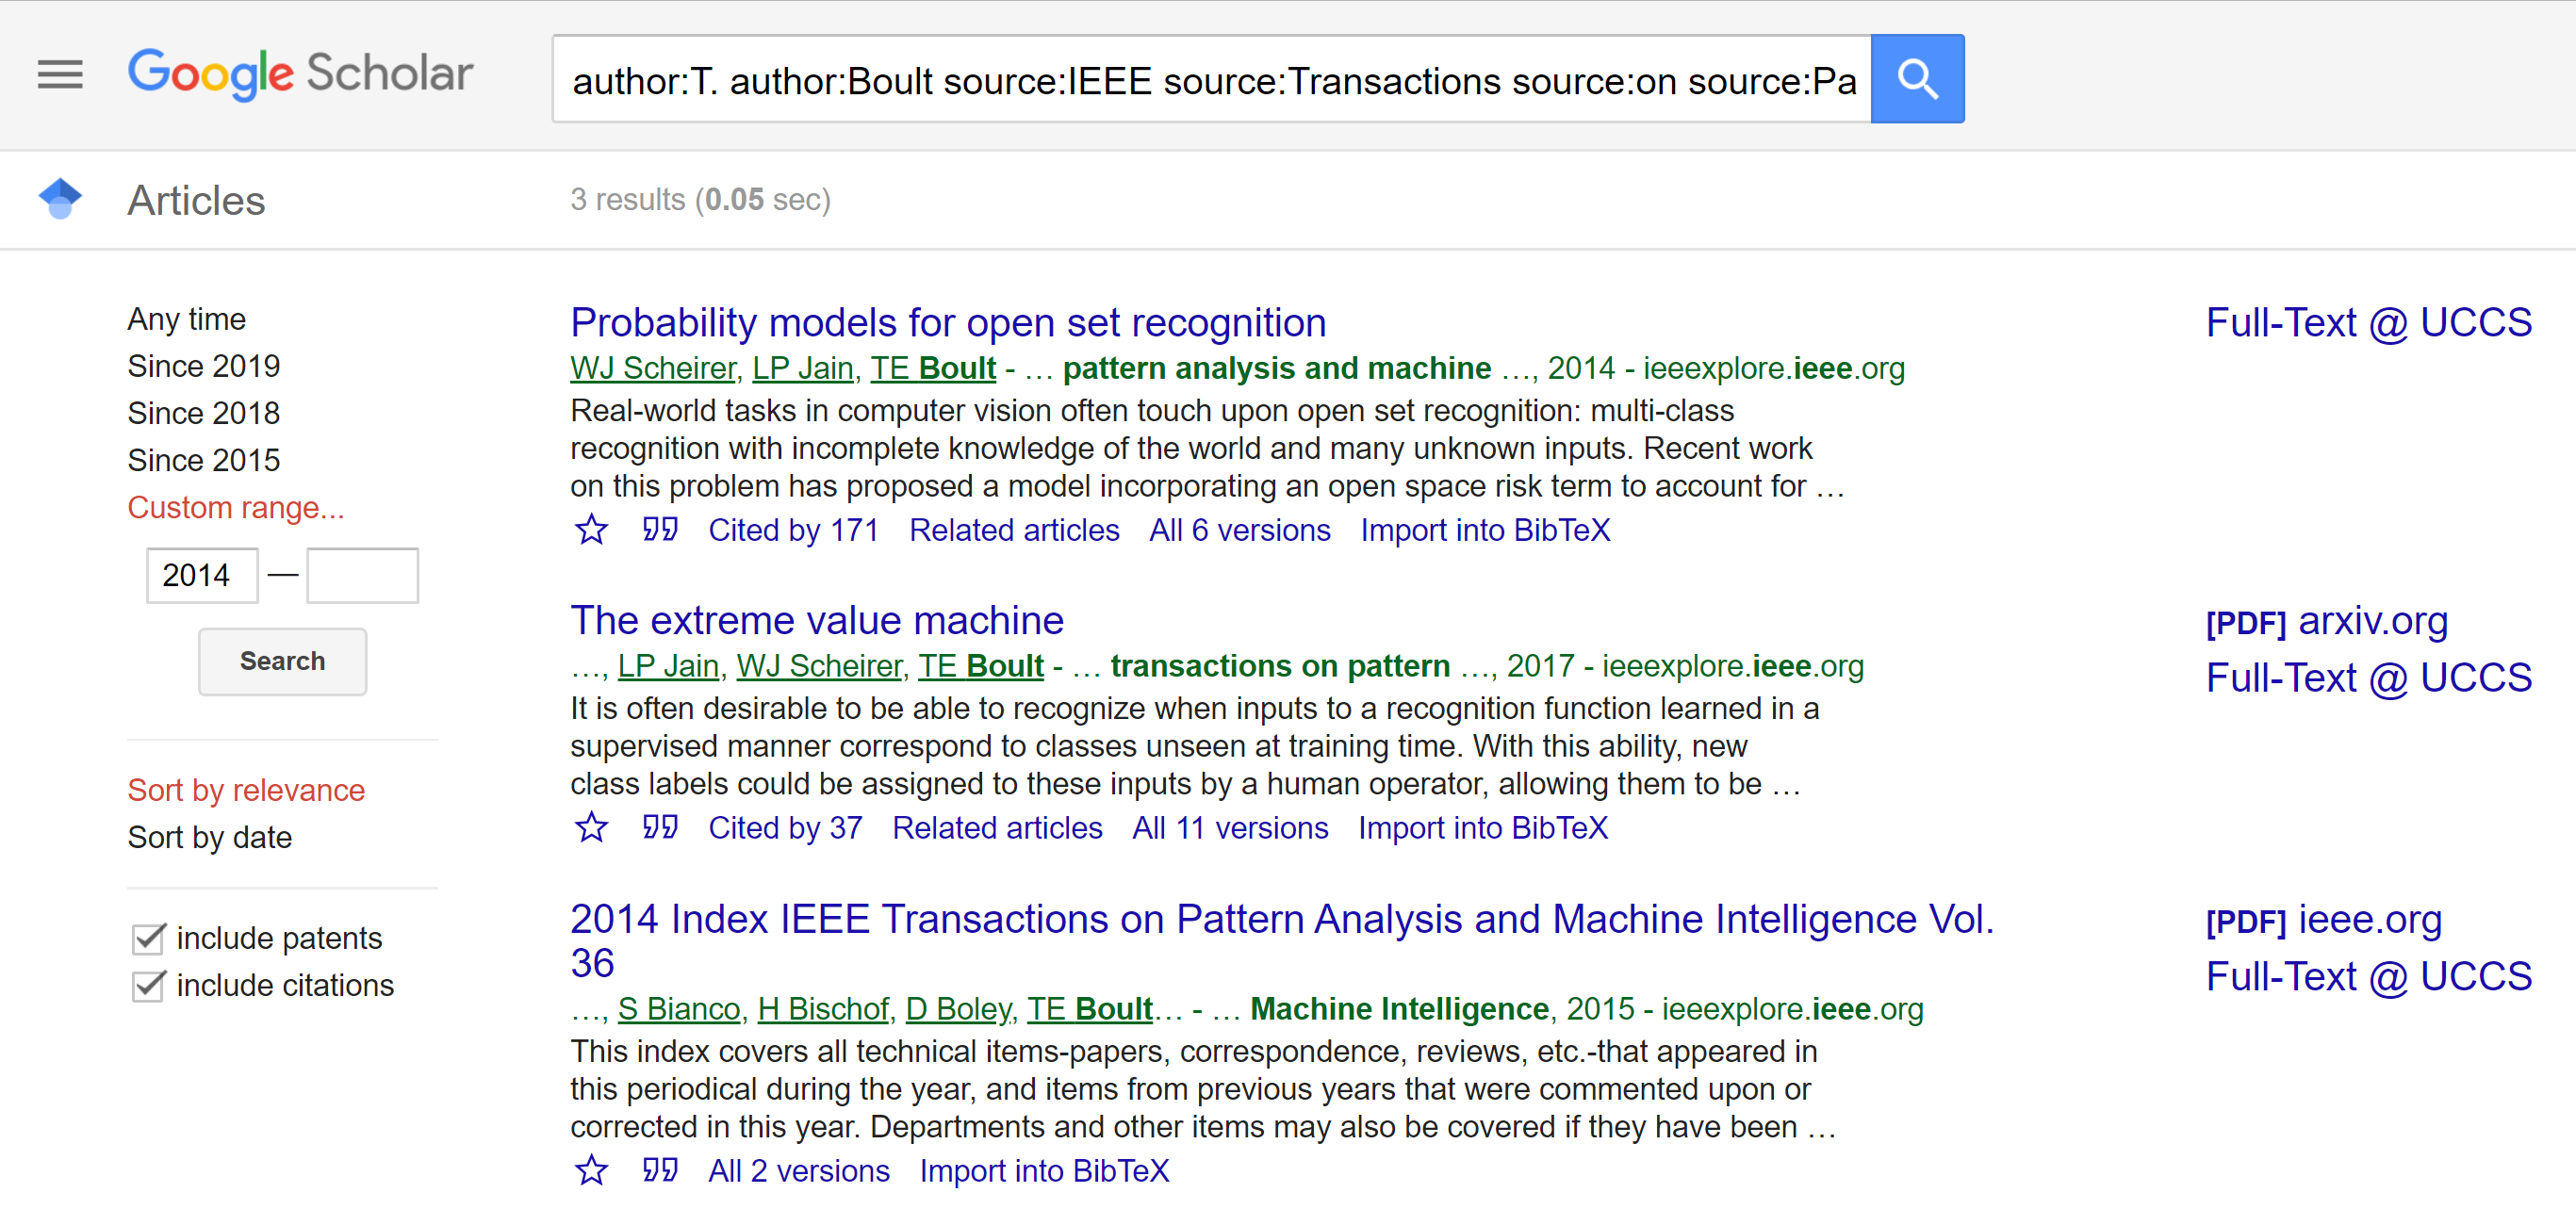
\includegraphics[width=0.9\linewidth]{images/fig5}
	\end{center}
	\captionsetup{labelformat=empty}
\end{figure}  

I pulled up the citation details \footnote{``2014 Index IEEE Transactions on Pattern Analysis and Machine Intelligence Vol. 36'' is an index into the authors who presented and the subjects that were presented in this particular conference. Hence, citation count of this index paper is irrelevant, for which the symbol N/A has been applied.} for the three papers above, which are provided below.  

\begin{center}
	\begin{tabular}{ |l|c|r| } 
		\hline
		{\footnotesize \textbf{Title}} & {\footnotesize \textbf{Cited by}} & {\footnotesize \textbf{Year}}\\
		\hline
		{\tiny Probability models for open set recognition \cite{article162}} & {\tiny 173} & {\tiny 2014} \\ 
		\hline
		{\tiny The extreme value machine \cite{article163}} & {\tiny 37} & {\tiny 2017} \\ 
		\hline
		{\tiny 2014 Index IEEE Trans. on Pattern Analysis and Machine Intelligence Vol. 36 \cite{article164}} & {\tiny N/A} & {\tiny 2015} \\ 
		\hline		
	\end{tabular}
\end{center} 

\vspace{5mm}

\bibliography{myref} 
\bibliographystyle{ieeetr}  

	
\end{document}